\documentclass[11pt]{article}

% === PACKAGES ===
\usepackage[a4paper, margin=1in]{geometry}
\usepackage{graphicx}
\usepackage{longtable}
\usepackage{array}
\usepackage{amsmath,amssymb}
\usepackage[utf8]{inputenc}
\usepackage[T1]{fontenc}
\usepackage{hyperref}
\usepackage{url}
\usepackage{booktabs}

% === HYPERREF SETUP ===
\hypersetup{
    colorlinks=true,
    linkcolor=blue,
    urlcolor=cyan,
}

% === DOCUMENT METADATA ===
\title{Benchmarking LLM Sensitivity to Prompt Formats: A Contamination-Free Approach}
\author{Fumio Miyata}
\date{}

% =================================
% === DOCUMENT START ===
% =================================
\begin{document}
\maketitle

\begin{abstract}
The evaluation of Large Language Models (LLMs) is complicated by prompt sensitivity and data contamination, which obscures the distinction between genuine reasoning and rote memorization. To address this, we introduce a reproducible, contamination-free benchmark that measures how LLM responses vary with the prompt's language, style, and syntactic format. Our methodology uses the constructed language Lojban---virtually absent from pre-training corpora---and a suite of novel symbolic prompting tasks to assess a model's ability to interpret unfamiliar formal systems. The results indicate three key findings: (1) prompt strictness can elicit latent capabilities, but its effectiveness is limited to familiar languages; (2) models exhibit a significant ceiling in algorithmic complexity, failing to produce bug-free code for novel tasks; and (3) performance appears more indicative of sophisticated pattern matching than abstract reasoning. This work provides a comprehensive dataset and a rigorous framework for evaluating the generalization and true reasoning abilities of LLMs.
\end{abstract}

\section{Introduction}
\label{sec:introduction}

Evaluating the capabilities of Large Language Models (LLMs) is a central challenge in modern AI research \cite{zhao2023survey}. While their performance is impressive, assessing it accurately is complicated by two well-documented issues: \textbf{Prompt Sensitivity}, where even subtle rephrasings can lead to vastly different outputs, and \textbf{Data Contamination}, where benchmark evaluation data is inadvertently included in a model's training set \cite{vaugrante2025prompt}. This contamination is a critical flaw in many public benchmarks, as it makes it difficult to determine if a model is demonstrating genuine reasoning or simply recalling a memorized answer.

The core of this problem is a gap in evaluation methodology. Existing benchmarks often cannot reliably test a model's ability to generalize to truly novel problems. To address this gap, our study introduces a new benchmark designed around the principle of data purity. We employ two primary strategies to create a contamination-free evaluation environment. First, we use the constructed language \textbf{Lojban}, a logical language with an unambiguous grammar virtually absent from pre-training corpora. Second, we developed \textbf{Symbolic Prompting}, a suite of custom tasks requiring the interpretation of formal rule sets in formats like S-expressions and JSON. This approach allows us to test a model's ability to adapt to unfamiliar formalisms, a closer proxy for genuine reasoning than performance on known benchmarks.

In this paper, we present the experimental framework, the resulting dataset, and a detailed analysis of our findings. We report on a series of experiments applying these prompts to a wide range of open-source LLMs. Our results suggest that (1) prompt format and strictness are critical factors in eliciting model capabilities, (2) models exhibit a clear ceiling when faced with complex, novel algorithmic implementation tasks, and (3) their performance is more consistent with sophisticated pattern-matching than with abstract reasoning. These findings have significant implications for how we should interpret LLM capabilities and design future evaluation methods.

\section{Experimental Environment}
\label{sec:environment}

\subsection{Setting up the Execution Environment}
To reproduce this experimental package, it is recommended to set up a Python virtual environment following the procedure described in the project's \texttt{README.md} file.

\subsection{Evaluated Models and Inference Parameters}
This study evaluates a range of open-source language models with fewer than 8 billion parameters, accessed via Ollama. The specific models and their inference hyperparameters are summarized in Table \ref{tab:models}.

\begin{table}[htbp]
\centering
\caption{Evaluated Models and Inference Hyperparameters}
\label{tab:models}
\begin{tabular}{@{}lccccc@{}}
\hline
Model Name (Ollama) & Parameters & Quant. (Est.) & Temp & Top P & Seed \\ \hline
\texttt{gemma3:270m}      & 0.27B      & Q4\_K\_M              & 0.0     & 1.0   & 0    \\ 
\texttt{smollm:360m}      & 0.36B      & Q4\_K\_M              & 0.0     & 1.0   & 0    \\ 
\texttt{qwen:0.5b}        & 0.5B       & Q4\_K\_M              & 0.0     & 1.0   & 0    \\ 
\texttt{tinyllama:1.1b}   & 1.1B       & Q4\_K\_M              & 0.0     & 1.0   & 0    \\ 
\texttt{deepseek-r1:1.5b} & 1.5B       & Unknown               & 0.0     & 1.0   & 0    \\ 
\texttt{stablelm2:1.6b}   & 1.6B       & Q4\_K\_M              & 0.0     & 1.0   & 0    \\ 
\texttt{qwen:1.8b}        & 1.8B       & Q4\_K\_M              & 0.0     & 1.0   & 0    \\ 
\texttt{gemma:2b}         & 2B         & Q4\_K\_M              & 0.0     & 1.0   & 0    \\ 
\texttt{falcon3:3b}       & 3B         & Unknown               & 0.0     & 1.0   & 0    \\ 
\texttt{llama3.2:3b}      & 3.2B       & Unknown               & 0.0     & 1.0   & 0    \\ 
\texttt{phi3:mini}        & 3.8B       & Q4\_K\_M              & 0.0     & 1.0   & 0    \\ 
\texttt{gemma3:4b}        & 4B         & Q4\_K\_M              & 0.0     & 1.0   & 0    \\ 
\texttt{qwen:4b}          & 4B         & Q4\_K\_M              & 0.0     & 1.0   & 0    \\ 
\texttt{yi:6b}            & 6B         & Q4\_K\_M              & 0.0     & 1.0   & 0    \\ 
\texttt{gemma:7b}         & 7B         & Q4\_K\_M              & 0.0     & 1.0   & 0    \\ 
\texttt{mistral:7b}       & 7B         & Q4\_K\_M              & 0.0     & 1.0   & 0    \\ 
\texttt{llama2:7b}        & 7B         & Q4\_K\_M              & 0.0     & 1.0   & 0    \\ 
\texttt{deepseek-llm:7b}  & 7B         & Q4\_K\_M              & 0.0     & 1.0   & 0    \\ 
\texttt{deepseek-r1:8b}   & 8B         & Unknown               & 0.0     & 1.0   & 0    \\ 
\texttt{llama3:8b}        & 8B         & Q4\_K\_M              & 0.0     & 1.0   & 0    \\ \hline
\end{tabular}
\end{table}

\emph{Note: Quantization methods are based on the Ollama library's defaults, typically \texttt{Q4\_K\_M} where specified. Details for some models marked 'Unknown' were not available.}

To ensure deterministic reproducibility, all experiments were conducted with inference hyperparameters fixed at \texttt{temperature: 0.0}, \texttt{top\_p: 1.0}, and \texttt{seed: 0}. This setup minimizes stochastic variations in model responses, allowing for a focused evaluation of the impact of the prompt format itself.

\subsection{Evaluation Criteria}
This benchmark defines task-specific success criteria as follows:

\textbf{Code Generation Tasks}: Success is defined as the generated Python code passing all predefined \texttt{Pytest} unit tests \textbf{without any modification}. Each task is attempted only once, making this a strict \textbf{Pass@1} evaluation.

\textbf{String Generation Task} (\texttt{filtered\_list}): Success requires that the list-formatted string returned by the model perfectly matches the expected output at the character level. This test evaluates the ability to follow instructions and adhere to a format directly, rather than generating code.

\textbf{Logical Reasoning Tasks}:
\begin{itemize}
    \item \textbf{Implementation Correctness}: Success is defined as the generated code correctly implementing the given logic (from S-expressions, JSON, a custom token language, etc.) and passing all associated unit tests.
    \item \textbf{Qualitative Analysis of Thought Process}: For tasks requiring Chain-of-Thought, the generated reasoning is qualitatively analyzed for faithfulness to the rules, logical consistency, and its influence on the final answer.
\end{itemize}

\section{Overview of Experimental Design}
\label{sec:design}

The benchmark comprises a suite of tasks that span from simple code generation to complex logical reasoning. For a complete description of each test, refer to the \texttt{README.md} file. This section highlights the conceptual design of four key experiments.

\subsection{Conceptual Diagrams of Each Test}
The following diagrams illustrate the workflows of the main tests in this benchmark.

\begin{figure}[htbp]
\centering
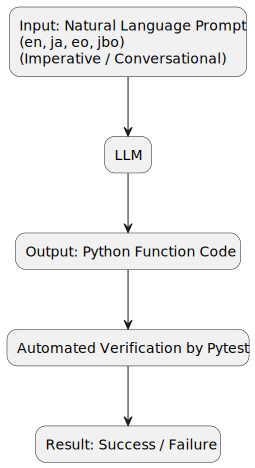
\includegraphics[width=0.6\textwidth]{figures/figure1_en.pdf}
\caption{Conceptual workflow for simple code generation tasks.}
\label{fig:fig1}
\end{figure}

\begin{figure}[htbp]
\centering
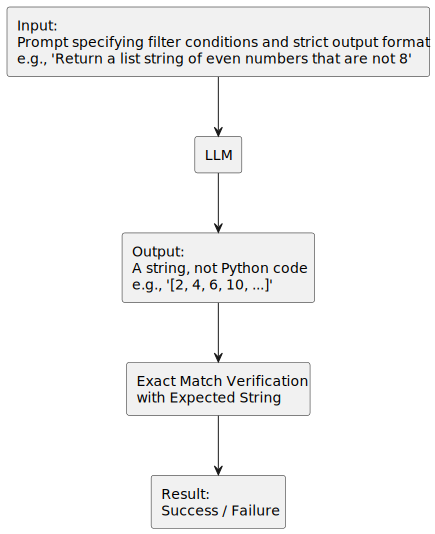
\includegraphics[width=0.6\textwidth]{figures/figure2_en.pdf}
\caption{Workflow for the \texttt{filtered\_list} task.}
\label{fig:fig2}
\end{figure}

\begin{figure}[htbp]
\centering
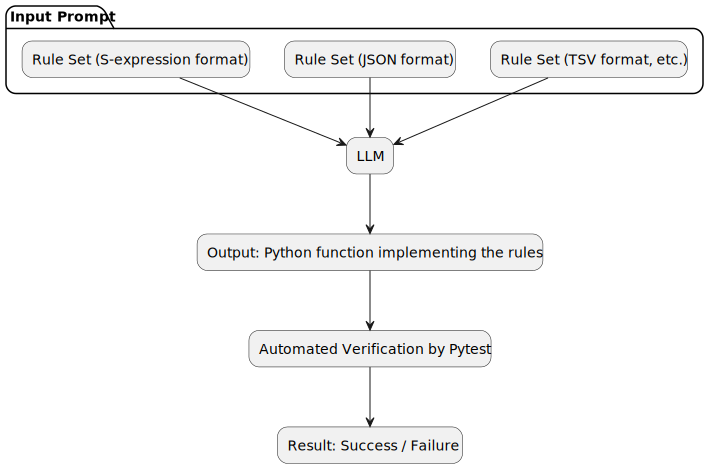
\includegraphics[width=0.8\textwidth]{figures/figure3_en.pdf}
\caption{Workflow for symbolic reasoning tasks.}
\label{fig:fig3}
\end{figure}

\begin{figure}[htbp]
\centering
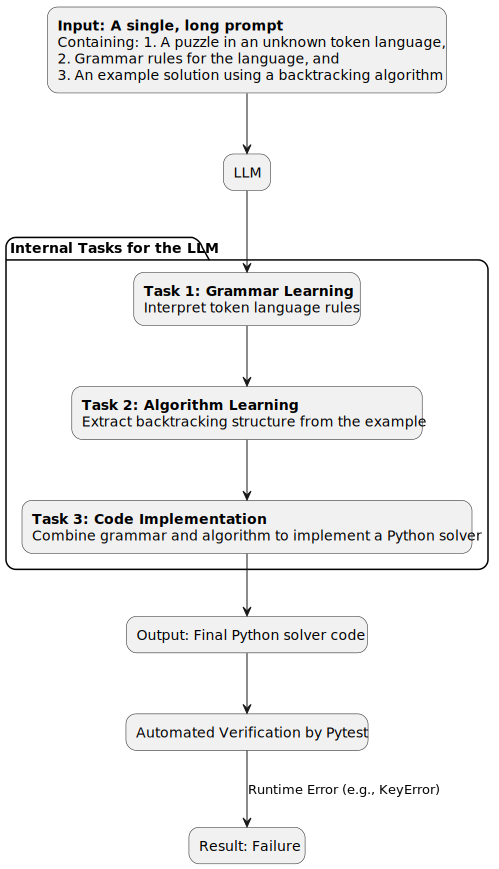
\includegraphics[width=0.7\textwidth]{figures/figure4_en.pdf}
\caption{Workflow for the \texttt{einstein\_token\_test} task.}
\label{fig:fig4}
\end{figure}


\section{Factual Results}
\label{sec:results}
This section presents the primary quantitative and qualitative results from the benchmark experiments. It is intentionally descriptive, reserving all interpretation for Section \ref{sec:discussion}. Full data tables for all 30 runs of each test are available in Appendix A.

\subsection{Outcome of the \texttt{Filtered List} Task}
The \texttt{Filtered List} task, which required models to return a formatted string rather than code, was executed under two conditions.
\begin{enumerate}
    \item \textbf{With an Ambiguous Prompt}: The initial prompt, which simply asked for a list, led most models to erroneously generate Python code that would produce the list.
    \item \textbf{With a Strict Prompt}: When the prompt was modified with a strict constraint---``Return only the list string, not a program code''---a significant number of models, including \texttt{deepseek-r1:8b} and \texttt{llama3:8b}, achieved high success rates for prompts in English and Japanese. For the same task in Lojban, however, all models failed, even with the strict constraint.
\end{enumerate}

\subsection{Observed Failure Pattern in the \texttt{einstein\_token\_test}}
The \texttt{einstein\_token\_test} confronted models with a multi-step reasoning task involving an unknown language. We observed a consistent, phased failure pattern:
\begin{enumerate}
    \item Given only the puzzle in the token language, no model produced comprehensible output.
    \item After adding the language's grammar rules to the prompt, some models attempted to generate Python code, but this code failed with \texttt{SyntaxError}.
    \item With the further addition of a few-shot example demonstrating a backtracking algorithm, models like \texttt{llama3:8b} produced syntactically valid code. However, this code failed at runtime, producing \texttt{KeyError} exceptions or timing out.
\end{enumerate}

\subsection{Performance on Symbolic vs. Natural Language Prompts}
In logical reasoning tasks such as \texttt{diagnosis}, models were prompted with rulesets in both natural language and symbolic formats. For some models, prompts using unambiguous symbolic languages like S-expressions and JSON yielded higher success rates than their natural language counterparts.

\subsection{Overall Performance and Model Scaling}
The aggregated results across all tests did not show a clear correlation between model parameter count and overall performance. As detailed in the rankings in Section \ref{subsec:performance}, several smaller models (e.g., \texttt{yi:6b}, \texttt{gemma3:4b}) outperformed larger ones.

\section{Discussion}
\label{sec:discussion}
In this section, we offer an interpretation of the factual results presented in Section \ref{sec:results}, discussing their potential implications for understanding LLM capabilities and evaluation.

\subsection{Interpretation of Prompt Strictness and Familiarity}
The results from the \texttt{Filtered List} test suggest that prompt strictness can be a crucial factor in eliciting correct model behavior. The dramatic performance improvement after adding a simple constraint indicates that models may possess latent abilities that are only unlocked when the expected output format is unambiguously specified.

However, this elicitation effect appears to be contingent on linguistic familiarity. The universal failure on the Lojban version of the same task suggests that the models did not leverage the language's unambiguous grammar for logical deduction. A plausible interpretation is that the models process unfamiliar languages like Lojban as sequences of unknown tokens, making them unable to perform the semantic task of mapping the language's logic to a specific output format. This asymmetry is consistent with phenomena like the ``Reversal Curse'' \cite{berglund2023reversal} and points to a potential broader issue of language understanding versus logical execution.

\subsection{Interpreting the Ceiling in Algorithmic Implementation}
The phased failure pattern in the \texttt{einstein\_token\_test} may indicate a ceiling in the ability of current LLMs to implement novel, complex algorithms. The final stage of failure---runtime errors in syntactically plausible code---is particularly revealing. A qualitative analysis of the code generated by \texttt{llama3:8b} highlights a potential cause: a failure to ensure state independence during recursion.

\begin{verbatim}
# Schematic excerpt of code generated by llama3:8b
def solve_puzzle(rules, assignments):
    # ...
    for value in domain_values(var):
        # The dictionary is mutated directly,
        # potentially leaking state across search paths.
        assignments[var] = value 
        if is_consistent(assignments, rules):
            result = solve_puzzle(rules, assignments)
            # ...
    # A backtracking step to undo the mutation is missing.
    return None
\end{verbatim}

One interpretation of this error is that while an LLM can imitate the superficial structure of an algorithm (loops, recursion), it may not be grasping the underlying logical requirements, such as state isolation in backtracking. This finding aligns with reported systematic failures in compositional reasoning and suggests that model abilities in this area may be confined to sophisticated pattern matching. It also contrasts with findings on Chain-of-Thought prompting, where including step-by-step reasoning can improve performance on complex tasks \cite{wei2022chain}, indicating that the format of reasoning is highly consequential.

\subsection{Interpreting the Effectiveness of Symbolic Interfaces}
The higher success rates on certain tasks when using symbolic prompts (S-expressions, JSON) suggest that these formats can serve as a more effective computational interface for LLMs in logically structured problems. Two factors may contribute to this: (1) \textbf{Syntactic Unambiguity}, which could reduce a model's interpretive overhead, and (2) \textbf{Token Efficiency}, which allows more complex logic to be represented concisely. This finding lends support to the potential value of hybrid symbolic-neural approaches for creating more reliable systems \cite{marcus2020next}.

\subsection{Interpreting Overall Performance and Lojban Failure}
\label{subsec:performance}
The lack of a clear correlation between model size and performance on our benchmark suggests that factors like architecture and training data composition may play a more significant role than parameter count alone for these specific reasoning tasks.

\begin{figure}[htbp]
\centering
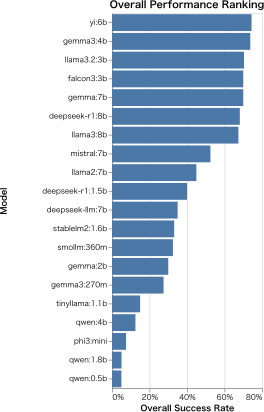
\includegraphics[width=0.8\textwidth]{figures/figure5_en.pdf}
\caption{Overall Performance Ranking.}
\label{fig:fig5}
\end{figure}

Furthermore, the consistent and near-total failure on Lojban tasks provides additional evidence that model performance may be rooted in pattern recognition rather than abstract reasoning. In a separate suite of basic Lojban translation tasks, all 20 models failed, suggesting the limited successes in the main benchmark were likely superficial ``transpilation'' of token patterns. One hypothesis is that this difficulty may originate at the tokenizer level, where Lojban's unique morphology could be fragmented into meaningless sub-tokens, thereby impeding the learning of word-level semantics.

\section{Limitations}
\label{sec:limitations}
This study's focus on lightweight, open-source models invites a comparative analysis with larger models (e.g., GPT-4, Claude 3). The algorithmic tests could also be expanded beyond backtracking to other complex tasks like dynamic programming to probe the generality of our findings. Finally, the use of deterministic generation parameters (\texttt{temperature: 0.0}) leaves room to explore how stochastic settings affect performance.

\section{Conclusion}
\label{sec:conclusion}
This paper presented a novel, contamination-free benchmark to probe the reasoning and implementation abilities of LLMs. Our experiments yielded several key observations: the effectiveness of prompt strictness appears contingent on linguistic familiarity; models may exhibit a ceiling in complex algorithmic implementation; and overall performance seems more rooted in pattern matching than abstract reasoning. These observations lend further support to the 'mirage' theory of emergent abilities \cite{schaeffer2023mirage}, which posits that such capabilities are a predictable outcome of scale, rather than an unpredictable 'emergence' of new abilities \cite{wei2022emergent}. We hope this framework contributes to a more nuanced evaluation of LLM capabilities and informs the future design of models that can reason more robustly.

\section{Ethical Considerations}
\label{sec:ethical}
This study highlights significant performance disparities in LLMs when prompted with non-mainstream languages like Lojban and Esperanto. These results suggest that current models are predominantly trained on data from mainstream languages such as English, creating a bias that risks the inadequate representation of other languages and cultures. From an ethical standpoint, our work underscores the need for greater diversity and inclusivity in the datasets used for future model development.

% 
% The manually formatted bibliography
% 
\begin{thebibliography}{99}

\bibitem{anam2025prompt}
Anam, M. (2025). \emph{Prompt Engineering and the Effectiveness of Large Language Models in Enhancing Human Productivity}. arXiv preprint arXiv:2507.18638.

\bibitem{berglund2023reversal}
Berglund, L., et al. (2023). The Reversal Curse: LLMs trained on \"A is B\" fail to learn \"B is A\". In \emph{Proceedings of the 12th International Conference on Learning Representations (ICLR 2024)}.

\bibitem{besta2023graph}
Besta, M., et al. (2023). Graph of Thoughts: Solving Elaborate Problems with Large Language Models. In \emph{Proceedings of the 12th International Conference on Learning Representations (ICLR 2024)}.

\bibitem{gao2022program}
Gao, L., et al. (2022). Program-Aided Language Models. In \emph{Proceedings of the 40th International Conference on Machine Learning (ICML)}, vol. 202, pp. 10764-10799. PMLR.

\bibitem{marcus2020next}
Marcus, G. (2020). \emph{The Next Decade in AI: Four Steps Towards Robust Artificial Intelligence}. arXiv preprint arXiv:2002.06177.

\bibitem{ronanki2025prompt}
Ronanki, S., et al. (2025). \emph{Prompt Engineering Guidelines for Using Large Language Models in Requirements Engineering}. arXiv preprint arXiv:2507.03405.

\bibitem{schaeffer2023mirage}
Schaeffer, R., et al. (2023). Are Emergent Abilities of Large Language Models a Mirage?. In \emph{Advances in Neural Information Processing Systems 36 (NeurIPS 2023)}.

\bibitem{thomas2023unsolvable}
Thomas, A. W., et al. (2023). \emph{Unsolvable Problems for Large Language Models: A Formal Language Approach}. arXiv preprint arXiv:2310.16799.

\bibitem{vaugrante2025prompt}
Vaugrante, L., et al. (2025). Prompt Engineering Techniques for Language Model Reasoning Lack Replicability. In \emph{Transactions on Machine Learning Research}.

\bibitem{wei2022chain}
Wei, J., et al. (2022a). Chain-of-Thought Prompting Elicits Reasoning in Large Language Models. In \emph{Advances in Neural Information Processing Systems 35 (NeurIPS 2022))}, pp. 24824–24837.

\bibitem{wei2022emergent}
Wei, J., et al. (2022b). Emergent Abilities of Large Language Models. In \emph{Transactions on Machine Learning Research}.

\bibitem{yao2023tree}
Yao, S., et al. (2023). Tree of Thoughts: Deliberate Problem Solving with Large Language Models. In \emph{Advances in Neural Information Processing Systems 36 (NeurIPS 2023)}.

\bibitem{zhao2023survey}
Zhao, W. X., et al. (2023). \emph{A Survey of Large Language Models}. arXiv preprint arXiv:2303.18223.

\end{thebibliography}

\appendix
\section{Appendix A: Detailed Experiment Results}
Below is a summary of the number of successful trials from a large-scale experiment with 30 runs for each test.

\tiny
\input{tables/return_one.tex}
\input{tables/copy_list.tex}
\input{tables/simple_sort.tex}
\input{tables/reverse_sort.tex}
\begin{longtable}{@{}lcccc@{}}
\caption{Length Sort Success Rates} \label{tab:length_sort} \\
\toprule
Model / Language & ja & en & eo & jbo \\
\midrule
\endfirsthead
\multicolumn{5}{c}{{\bfseries \tablename\ \thetable{} -- continued from previous page}} \\\toprule
Model / Language & ja & en & eo & jbo \\
\midrule
\endhead
\bottomrule
\endfoot
\texttt{gemma3:270m} & 30/30 & 30/30 & 0/30 & 0/30 \\
\texttt{smollm:360m} & 30/30 & 30/30 & 30/30 & 30/30 \\
\texttt{qwen:0.5b} & 0/30 & 0/30 & 0/30 & 0/30 \\
\texttt{tinyllama:1.1b} & 0/30 & 0/30 & 0/30 & 0/30 \\
\texttt{deepseek-r1:1.5b} & 30/30 & 30/30 & 0/30 & 0/30 \\
\texttt{stablelm2:1.6b} & 0/30 & 30/30 & 29/30 & 0/30 \\
\texttt{qwen:1.8b} & 0/30 & 0/30 & 0/30 & 0/30 \\
\texttt{gemma:2b} & 0/30 & 0/30 & 0/30 & 0/30 \\
\texttt{falcon3:3b} & 0/30 & 30/30 & 30/30 & 30/30 \\
\texttt{llama3.2:3b} & 30/30 & 30/30 & 30/30 & 30/30 \\
\texttt{phi3:mini} & 0/30 & 0/30 & 0/30 & 0/30 \\
\texttt{gemma3:4b} & 30/30 & 30/30 & 30/30 & 30/30 \\
\texttt{qwen:4b} & 0/30 & 0/30 & 0/30 & 0/30 \\
\texttt{yi:6b} & 30/30 & 30/30 & 30/30 & 0/30 \\
\texttt{gemma:7b} & 30/30 & 30/30 & 30/30 & 0/30 \\
\texttt{mistral:7b} & 30/30 & 29/30 & 30/30 & 0/30 \\
\texttt{llama2:7b} & 0/30 & 30/30 & 30/30 & 30/30 \\
\texttt{deepseek-llm:7b} & 0/30 & 30/30 & 30/30 & 0/30 \\
\texttt{deepseek-r1:8b} & 30/30 & 30/30 & 30/30 & 30/30 \\
\texttt{llama3:8b} & 30/30 & 30/30 & 30/30 & 30/30 \\
\end{longtable}

\input{tables/custom_sort.tex}
\begin{longtable}{@{}lc@{}}
\caption{Roundtrip (Fibonacci S-Expr) Success Rates} \label{tab:roundtrip_fibonacci} \\
\toprule
Model / Format & sexpr \\
\midrule
\endfirsthead
\multicolumn{2}{c}{{\bfseries \tablename\ \thetable{} -- continued from previous page}} \\\toprule
Model / Format & sexpr \\
\midrule
\endhead
\bottomrule
\endfoot
\texttt{gemma3:270m} & 0/30 \\
\texttt{smollm:360m} & 0/30 \\
\texttt{qwen:0.5b} & 0/30 \\
\texttt{tinyllama:1.1b} & 0/30 \\
\texttt{deepseek-r1:1.5b} & 0/30 \\
\texttt{stablelm2:1.6b} & 0/30 \\
\texttt{qwen:1.8b} & 0/30 \\
\texttt{gemma:2b} & 0/30 \\
\texttt{falcon3:3b} & 0/30 \\
\texttt{llama3.2:3b} & 0/30 \\
\texttt{phi3:mini} & 0/30 \\
\texttt{gemma3:4b} & 30/30 \\
\texttt{qwen:4b} & 0/30 \\
\texttt{yi:6b} & 23/30 \\
\texttt{gemma:7b} & 0/30 \\
\texttt{mistral:7b} & 30/30 \\
\texttt{llama2:7b} & 0/30 \\
\texttt{deepseek-llm:7b} & 0/30 \\
\texttt{deepseek-r1:8b} & 8/30 \\
\texttt{llama3:8b} & 0/30 \\
\end{longtable}

\begin{longtable}{@{}lcccc@{}}
\caption{Diagnosis Logic Success Rates} \label{tab:diagnosis_logic} \\
\toprule
Model / Format & S-expression & json & tsv & token-test \\
\midrule
\endfirsthead
\multicolumn{5}{c}{{\bfseries \tablename~\thetable{} -- continued from previous page}} \\
\toprule
Model / Format & S-expression & json & tsv & token-test \\
\midrule
\endhead
\bottomrule
\endfoot
\texttt{gemma3:270m} & 0/30 & 0/30 & 0/30 & 0/30 \\
\texttt{smollm:360m} & 0/30 & 0/30 & 0/30 & 0/30 \\
\texttt{qwen:0.5b} & 0/30 & 0/30 & 0/30 & 0/30 \\
\texttt{tinyllama:1.1b} & 0/30 & 0/30 & 0/30 & 0/30 \\
\texttt{deepseek-r1:1.5b} & 30/30 & 0/30 & 0/30 & 0/30 \\
\texttt{stablelm2:1.6b} & 28/30 & 0/30 & 0/30 & 4/30 \\
\texttt{qwen:1.8b} & 0/30 & 0/30 & 0/30 & 0/30 \\
\texttt{gemma:2b} & 30/30 & 0/30 & 30/30 & 30/30 \\
\texttt{falcon3:3b} & 30/30 & 30/30 & 30/30 & 0/30 \\
\texttt{llama3.2:3b} & 30/30 & 30/30 & 5/30 & 30/30 \\
\texttt{phi3:mini} & 0/30 & 0/30 & 0/30 & 0/30 \\
\texttt{gemma3:4b} & 30/30 & 30/30 & 30/30 & 30/30 \\
\texttt{qwen:4b} & 0/30 & 0/30 & 0/30 & 0/30 \\
\texttt{yi:6b} & 30/30 & 0/30 & 30/30 & 30/30 \\
\texttt{gemma:7b} & 30/30 & 30/30 & 30/30 & 30/30 \\
\texttt{mistral:7b} & 0/30 & 0/30 & 0/30 & 30/30 \\
\texttt{llama2:7b} & 0/30 & 0/30 & 0/30 & 30/30 \\
\texttt{deepseek-llm:7b} & 0/30 & 0/30 & 0/30 & 30/30 \\
\texttt{deepseek-r1:8b} & 29/30 & 1/30 & 1/30 & 0/30 \\
\texttt{llama3:8b} & 30/30 & 30/30 & 30/30 & 30/30 \\
\end{longtable}

\input{tables/einstein_symbolic.tex}
\begin{longtable}{@{}lcccc@{}}
\caption{Einstein Riddle Success Rates (CoT Formats)} \label{tab:einstein_cot} \\
\toprule
Model & CoT (ja) & CoT (en) & CoT (eo) & CoT (jbo) \\
\midrule
\endfirsthead
\multicolumn{5}{c}{{\bfseries \tablename~\thetable{} -- continued from previous page}} \\
\toprule
Model & CoT (ja) & CoT (en) & CoT (eo) & CoT (jbo) \\
\midrule
\endhead
\bottomrule
\endfoot
\texttt{gemma3:270m} & 30/30 & 30/30 & 0/30 & 30/30 \\
\texttt{smollm:360m} & 0/30 & 0/30 & 0/30 & 0/30 \\
\texttt{qwen:0.5b} & 0/30 & 0/30 & 0/30 & 0/30 \\
\texttt{tinyllama:1.1b} & 0/30 & 0/30 & 0/30 & 0/30 \\
\texttt{deepseek-r1:1.5b} & 0/30 & 0/30 & 0/30 & 0/30 \\
\texttt{stablelm2:1.6b} & 0/30 & 7/30 & 4/30 & 3/30 \\
\texttt{qwen:1.8b} & 0/30 & 0/30 & 0/30 & 0/30 \\
\texttt{gemma:2b} & 0/30 & 0/30 & 30/30 & 0/30 \\
\texttt{falcon3:3b} & 30/30 & 0/30 & 30/30 & 0/30 \\
\texttt{llama3.2:3b} & 0/30 & 0/30 & 0/30 & 30/30 \\
\texttt{phi3:mini} & 0/30 & 0/30 & 0/30 & 0/30 \\
\texttt{gemma3:4b} & 0/30 & 30/30 & 0/30 & 0/30 \\
\texttt{qwen:4b} & 0/30 & 0/30 & 0/30 & 0/30 \\
\texttt{yi:6b} & 0/30 & 0/30 & 0/30 & 30/30 \\
\texttt{gemma:7b} & 0/30 & 30/30 & 0/30 & 0/30 \\
\texttt{mistral:7b} & 0/30 & 0/30 & 0/30 & 1/30 \\
\texttt{llama2:7b} & 30/30 & 0/30 & 30/30 & 0/30 \\
\texttt{deepseek-llm:7b} & 0/30 & 0/30 & 0/30 & 0/30 \\
\texttt{deepseek-r1:8b} & 0/30 & 0/30 & 0/30 & 0/30 \\
\texttt{llama3:8b} & 0/30 & 0/30 & 30/30 & 0/30 \\
\end{longtable}
\input{tables/filtered_list.tex}

\end{document}
